\documentclass{article}
\usepackage[T1]{fontenc}
\usepackage{lmodern}
\usepackage{graphicx}
\usepackage{amsmath,amssymb}
\usepackage[a4paper,margin=2cm]{geometry}
\usepackage[absolute,overlay]{textpos}
\setlength{\TPHorizModule}{1mm}
\setlength{\TPVertModule}{1mm}
\usepackage[indonesian]{babel}
\usepackage{hyperref}
\setlength{\emergencystretch}{2em}
% unit: Halaman 35

\begin{document}

% === Halaman 35 (llm) ===

\textcolor{red}{Plainteks:}\vspace{2mm}
\begin{center}
\fbox{\parbox{0.6\textwidth}{Dinas Pendidikan Kota Ternate meminta kepada pihak sekolah dan orang tua siswa untuk jenjang pendidikan SD dan SMP se-Kota Ternate untuk melarang para siswa membawa permainan lato-lato yang sedang tren itu ke sekolah, karena akan mengganggu kegiatan belajar mengajar yang dinilai berbahaya sehingga mengantisipasi kecelakaan bagi anak di daerah itu.}}
\end{center}

\vspace{10mm}

\textcolor{red}{Cipherteks:}\vspace{2mm}
\begin{center}
\fbox{\parbox{0.6\textwidth}{HAWFHZDOHAHANGOMKLGF CVWFLBOCPRKFGNHOFNIN\\SPGNLHMPFVBEFWMVFWTBWRHSFZRWK FQMVHPAFWIK\\DOHAHANGPFEWNFPNFKNLHMPFGLBAMGFCXK FQ MOCFV\\AVKANIAVHSFZRN CODGAFOHYUVGWFOFGFXEG FMLFWIT\\HEFWTBVCPAYQOBLHMPFVBPVADOVWGN FWOCKARVKA\\RQOBRGGFFWCHFVGYUDORVGVYCFWABAPVSVGCHGCI\\DRFIFHBAPVQRVOCKAFWSGHSNIHSOBDHFVNGFWDGRGF\\WGNHANFCVIDGSWZ}}
\end{center}

% deskripsi: Kotak berisi teks plainteks dalam Bahasa Indonesia mengenai larangan permainan lato-lato di sekolah.
% bbox normalisasi: [0.2270, 0.3400, 0.8270, 0.4640]
\begin{textblock*}{126.00mm}(47.67mm,100.98mm)
\noindent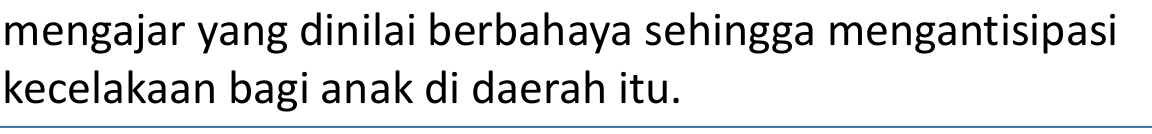
\includegraphics[width=126.00mm,height=36.83mm]{../../images/llm/page_035_img_01.png}%
\end{textblock*}

% deskripsi: Kotak berisi teks cipherteks yang terdiri dari rangkaian huruf kapital acak.
% bbox normalisasi: [0.2270, 0.5110, 0.8270, 0.9530]
\begin{textblock*}{126.00mm}(47.67mm,151.77mm)
\noindent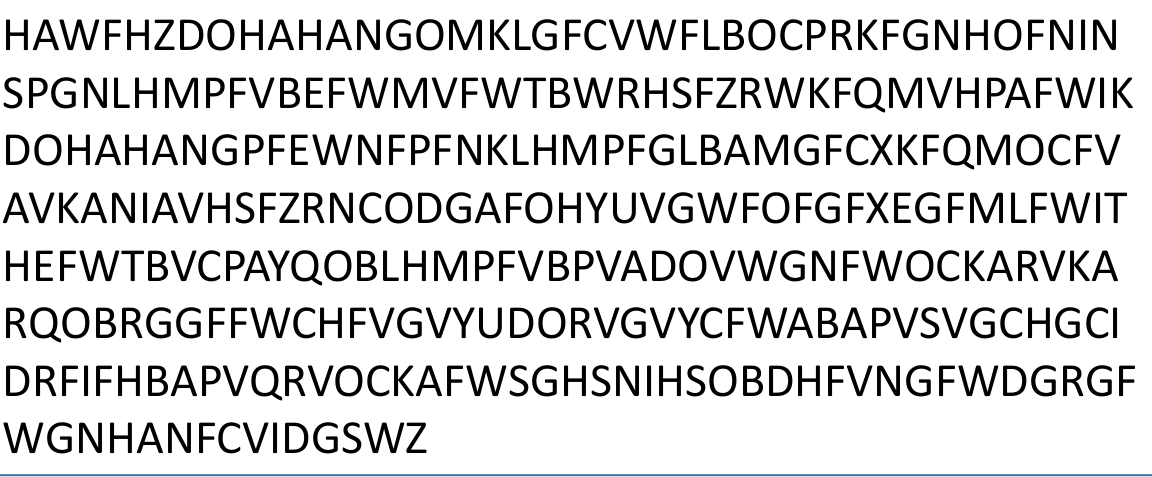
\includegraphics[width=126.00mm,height=131.27mm]{../../images/llm/page_035_img_02.png}%
\end{textblock*}

\end{document}
